\documentclass[options]{article}

% para que traduzca las cosas por defecto del programa a español (ej: abstract -> resumen)
\usepackage[spanish]{babel}
% para insertar imágenes
\usepackage{graphicx}
% para poner headers a las tablas
\usepackage{makecell}
\renewcommand\theadfont{\bfseries\sffamily}

% para meter subtítulos grado 4
\usepackage{titlesec}
\setcounter{secnumdepth}{4}
\titleformat{\paragraph}
{\normalfont\normalsize\bfseries}{\theparagraph}{1em}{}
\titlespacing*{\paragraph}
{0pt}{3.25ex plus 1ex minus .2ex}{1.5ex plus .2ex}

% para que las figuras no aparezcan siempre en el top de la página
\usepackage{float}

% para que el toc tenga los links
\usepackage{hyperref}
\hypersetup{
    colorlinks=true, %set true if you want colored links
    linktoc=all,     %set to all if you want both sections and subsections linked
    linkcolor=black,  %choose some color if you want links to stand out
}

\title{Práctica del Tema 5: Publicación y difusión}
\author{Blanca María Pérez Soriano}

\begin{document}
\maketitle

\pagebreak

\tableofcontents

\pagebreak

\section{Introducción}
Creación y publicación de un modelo 3D a partir de un modelo digitalizado representado como una nube de puntos

% TODO: meter todas las imágenes en figuras
% TODO: ajustar las tablas e imágenes a las sangrías
% TODO: revisar los caption de las imágenes

\section{Metodología empleada}
\subsection{Software}
Para realizar esta práctica utilizaremos el programa \href{https://www.meshlab.net/}{MeshLab} en la versión 64bit v2023.12.
\subsection{Modelo de puntos}
Para la realización de esta práctica se utilizará el modelo de nube puntos proporcionado en el recurso \textit{``Modelos para la práctica"}: \textbf{MayanSculpture.ply}.
\subsection{Importación a MeshLab}

Para importar el modelo de nube de puntos seleccionado seguiremos las siguientes acciones: \textbf{File → Import Mesh → MayanSculpture.ply}
\begin{center}
    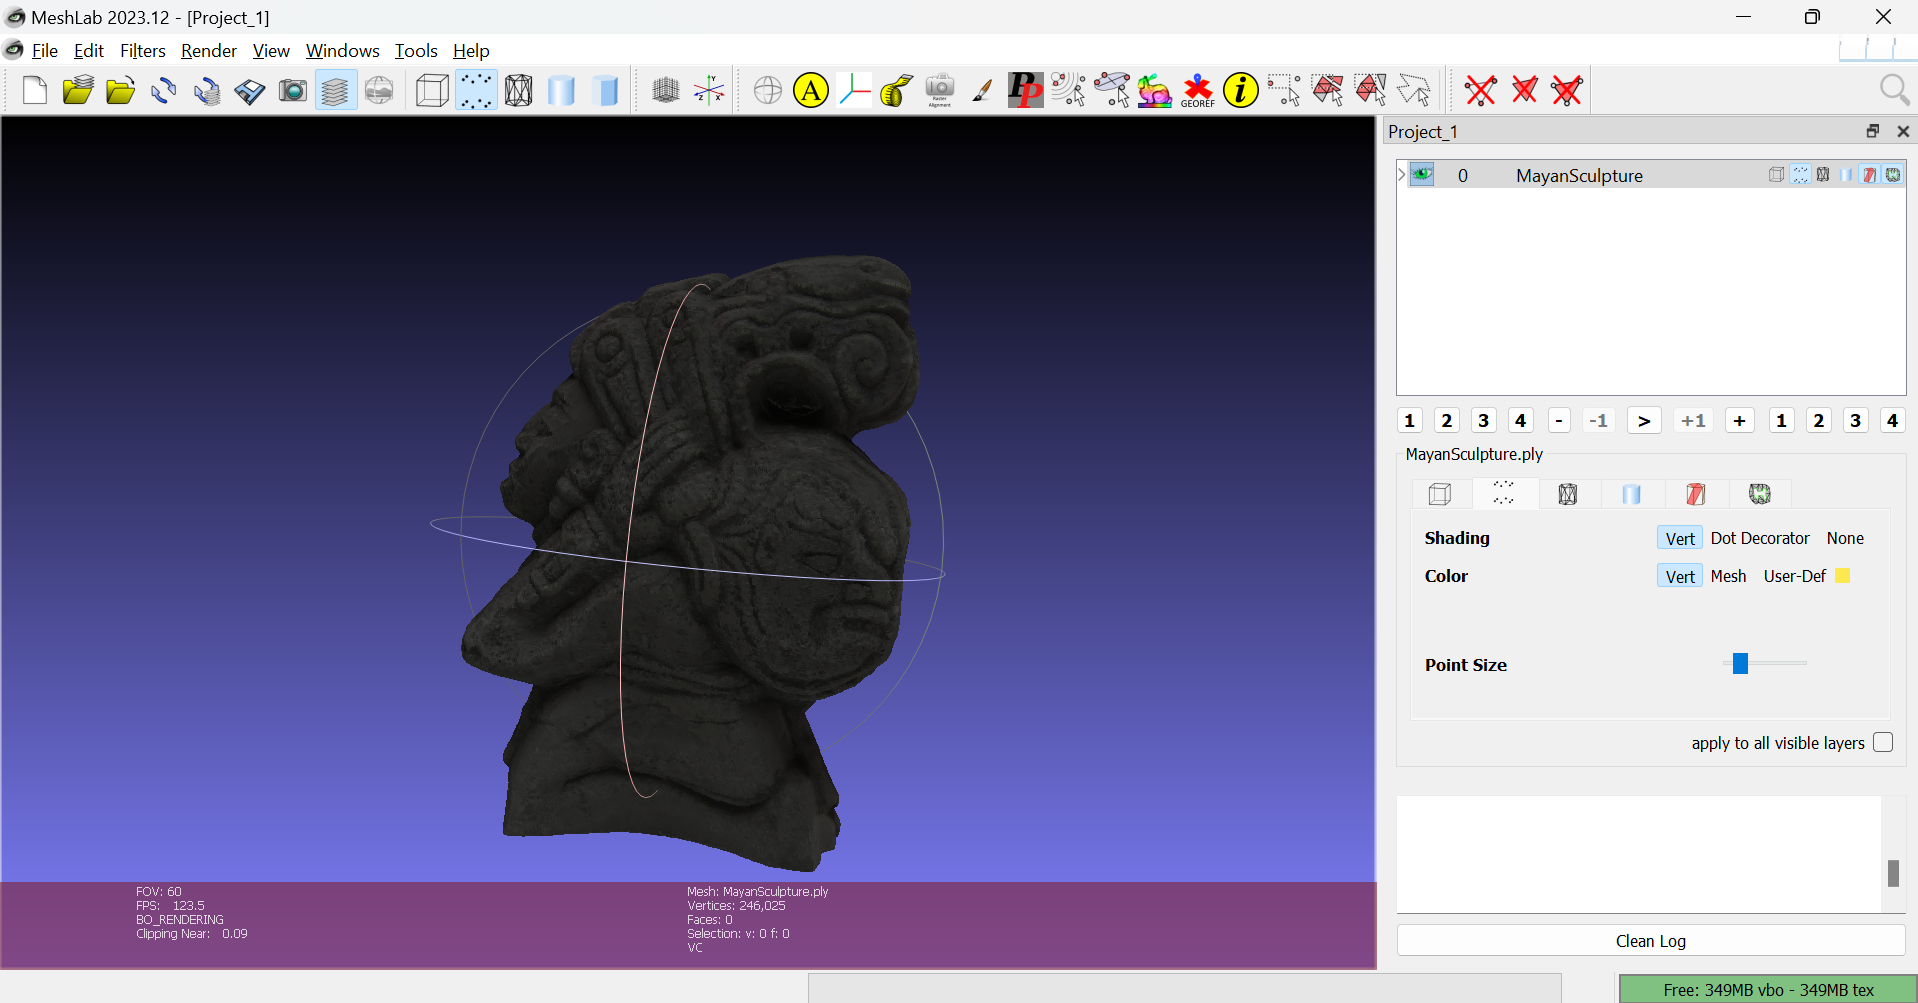
\includegraphics[scale=0.35]{images/presentacion_importacion.png}    
\end{center}

Es una malla de 246.025 vértices y no tiene caras.
\pagebreak

\section{Resolución de la práctica}
\subsection{Shading}

Para empezar correctamente, lo primero que haremos será intentar mejorar el \textit{shading} de la pieza. Para ello calcularemos las normales, esto hará que los puntos de luz sean tomados perpendicularmente. Deberemos hacer click en la siguiente secuencia: \textbf{Filters → Point Set → compute normals for point sets}. Tras esto, se nos desplegará la siguiente ventana, deberemos hacer click en \textit{``Apply''}:

\begin{center}
    \includegraphics[scale=0.65]{images/triangulación_01.png}    
\end{center}

Ahora podemos ver el claro cambio de color y trazado en la pieza:
\begin{center}
    \includegraphics[scale=0.35]{images/triangulación_02.png}    
\end{center}

\subsection{Triangulación}
% TODO: breve explicación de lo que es triangular y para qué sirve

\subsubsection{Reconstrucción de la superficie mediante Screened Poisson}
Para ello hacemos click en: \textbf{\textit{``Filters → Remeshing, Simplification and Reconstruction → Surface Reconstruction: Screened Poisson''}}. Se nos desplegará la siguiente ventana:

\begin{center}
    \includegraphics[scale=0.65]{images/triangulación_03.png}    
\end{center}

De esta ventana, los dos valores interesantes son:
\begin{itemize}
    \item \textbf{Reconstruction Depth}: este valor lo retocaremos en base a la pérdida o ganancia de puntos tras la reconstrucción.
    \item \textbf{Pre-Clean}: Este \textit{checkbox} haría un prelimpiado de normales con valores nulos, en caso de ser marcado.
\end{itemize}

Como hemos visto en el curso, un buen valor de \textbf{Reconstruction Depth} para lanzar una primera reconstrucción sería el \textbf{8}. De manera que lanzamos la reconstrucción sin tocar nada más y vemos si tenemos que reajustar. El resultado fue el siguiente:

\pagebreak

\begin{figure}[H]
    \centering
    \includegraphics[scale=0.40]{images/triangulación_04.png}
    \caption{Reconstrucción sin pre-clean}
\end{figure}

\begin{itemize}
    \item \textbf{vértices:} 135.855
    \item \textbf{caras:} 271.706
\end{itemize}

\begin{figure}[H]
    \centering       
    \includegraphics[scale=0.40]{images/triangulación_05.png}
    \caption{Reconstrucción con pre-clean}
\end{figure}

\pagebreak

\begin{itemize}
    \item \textbf{vértices:} 135.855
    \item \textbf{caras:} 271.706
\end{itemize}

La malla original tenía 246.025 puntos, de manera que hemos reducido casi en la mitad la calidad del modelo. Podemos observar, si nos acercamos a la pieza, este tipo de pérdidas:
\begin{center}
    \begin{tabular}{|l|}
        \hline
        \thead{Por puntos} \\
        \hline
        \includegraphics[scale=0.40]{images/triangulación_06.png} \\
        \hline
        \thead{Poisson Mesh} \\
        \hline
        \includegraphics[scale=0.40]{images/triangulación_07.png} \\
        \hline
    \end{tabular}
\end{center}

\pagebreak

Repetimos el proceso aumentando el nivel de profundidad en 1. El resultado es el siguiente:
\begin{center}
    \begin{tabular}{|l|}
        \hline
        \thead{Por puntos} \\
        \hline
        \includegraphics[scale=0.40]{images/triangulación_08.png} \\
        \hline
        \thead{Poisson Mesh} \\
        \hline
        \includegraphics[scale=0.40]{images/triangulación_09.png} \\
        \hline
    \end{tabular}
\end{center}

Esta vez se han generado 546.859 vértices. A partir de aquí podríamos cambiar el color de la pieza, pero la verdad es que me gusta cómo está quedando. 

\pagebreak

Si hubiera querido cambiarlo, me habría movido entre estas dos pestañas del panel derecho, siendo la primera señalada la de los vértices y la segunda señalada la de las caras:

\begin{center}
    \includegraphics[scale=0.65]{images/triangulación_10.png}    
\end{center}

Finalmente queda eliminar algún triángulo artificial. Para ello hacemos click en \textbf{\textit{Filters → Selection → Select faces with edges larger than...}}, y el valor promedio para esta pieza es de 0.795821:

\begin{center}
    \includegraphics[scale=0.65]{images/triangulación_11.png}    
\end{center}

Tras darle a \textit{``Apply''} veo que sólo 6 caras son seleccionadas, por lo que no tocaremos nada más de momento:

\begin{center}
    \includegraphics[scale=0.65]{images/triangulación_12.png}    
\end{center}
\subsubsection{Corrección topológica de la malla}

Habiendo guardado una copia de la malla triangulada generada y habiendo eliminado la malla de nube de puntos, duplico la malla triangulada dentro del programa para prevenirnos del efecto de malas acciones, y empezamos con las técnicas.

\paragraph{Autointersecciones}
Para detectar \textbf{autointersecciones} hacemos clicks en los siguientes apartados: \textbf{\textit{Filters → Selection → Select self intersecting faces}}. Tras este proceso, veo que no se han seleccionado caras por lo que no aplico ninguna eliminación:

\begin{center}
    \includegraphics[scale=0.6]{images/triangulación_13.png}    
\end{center}

\pagebreak

\paragraph{Elementos no-variedad}

\begin{figure}[H]
    \centering
    \includegraphics[scale=0.65]{images/triangulación_14.png}
    \caption{Aristas no-variedad}
\end{figure}

\begin{figure}[H]
    \centering
    \includegraphics[scale=0.65]{images/triangulación_15.png}    
    \caption{Vértices no-variedad}
\end{figure}

No sale nada para ninguno de los dos, así que parece todo perfecto por ahora.

\paragraph{T-Vértices}

Para limpiar los vértices que conectan con el punto interior de una arista haremos click en \textbf{\textit{Filters → Cleaning \& Repairing → Remove T-Vertices}}, nos saldrá un panel y deberemos hacer click en \textit{``Apply''}. Para este caso sí nos han salido unas poquitas ocurrencias:


\begin{figure}[H]
    \centering
    \includegraphics[scale=0.6]{images/triangulación_16.png}
    \caption{Panel de T-Vértices}
\end{figure}


\begin{figure}[H]
    \centering
    \includegraphics[scale=1]{images/triangulación_17.png} 
    \caption{Log}
\end{figure}

\paragraph{Filtrados varios}

En este apartado dejaré fotos de algunos fitrados más que se han hecho antes del tapado de fisuras:

\begin{figure}[H]
    \centering
    \includegraphics[scale=0.75]{images/triangulación_18.png}
    \caption{Panel de T-Vértices}
\end{figure}

\begin{figure}[H]
    \centering
    \includegraphics[scale=0.75]{images/triangulación_19.png}
    \caption{Panel de T-Vértices}
\end{figure}
\begin{figure}[H]
    \centering
    \includegraphics[scale=0.75]{images/triangulación_20.png}
    \caption{Panel de T-Vértices}
\end{figure}

\paragraph{Tapado de fisuras}

Una vez tenemos la malla limpia, procedemos a tapar posibles agujeros. Para ello vamos a \textbf{\textit{Filters → Remeshing, Simplification and Reconstruction → Close Holes}}. Se nos desplegará el siguiente panel:

\begin{figure}[H]
    \centering
    \includegraphics[scale=0.75]{images/triangulación_21.png}
    \caption{Panel de T-Vértices}
\end{figure}

\begin{figure}[H]
    \centering
    \includegraphics[scale=0.75]{images/triangulación_22.png}
    \caption{Panel de T-Vértices}
\end{figure}

Parece que no se ha tapado ningún hueco. Tras esto, estuve probando distintos valores de aristas a tapar, oscilando entre 20 y 70, pero no obtuve otro mensaje en el log, así que parece una malla bastante sólida.

Si se hubieran generado nuevas caras y vértices, habría que repetir todo este proceso de nuevo \textit{(comprobar autointersecciones, eliminar elementos no-variedad, eliminar t-vértices, etc)}, para asegurar que la malla queda limpia.

\subsection{Simplificación}

Para agilizar la publicación de nuestro modelo en los medios, es posible que necesitemos reducir su tamaño intentando mantener su aspecto visual, esto puede conseguirse reduciendo el número de vértices y triángulos del modelo.

\subsubsection{Simplificación: Quadratic Edge Collapse Decimation}

Vamos a elegir este algoritmo por ser el que más respeta los detalles, dentro de lo que hemos visto en el curso. Para ello hacemos click en las siguientes secciones: \textbf{\textit{Filters → Remeshing, Simplification and Reconstruction → Simplification: Quadratic Edge Collapse Decimation}}:

\begin{figure}[H]
    \centering
    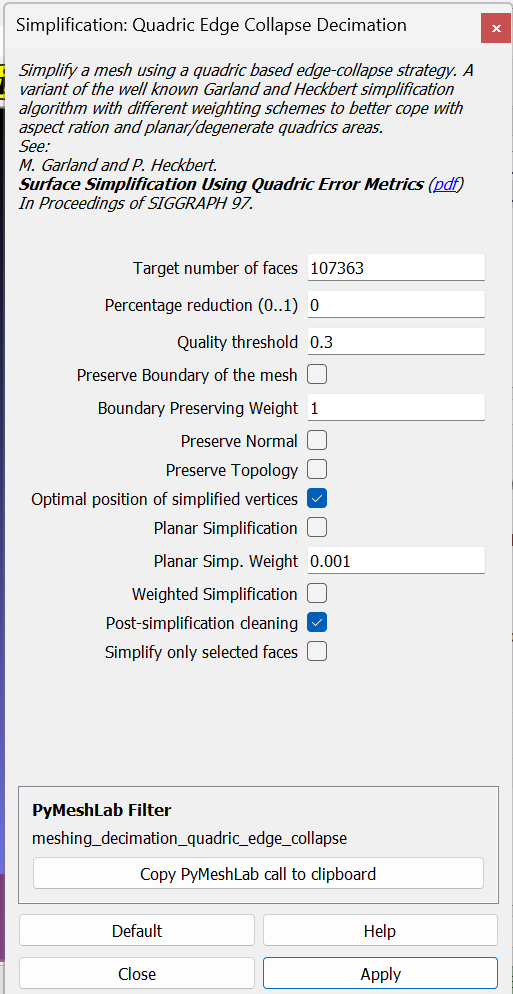
\includegraphics[scale=0.75]{images/simplificacion_01.png}
    \caption{Panel de Simplificación: Quadratic Edge Collapse Decimation}
\end{figure}

Como es requisito de esta práctica entregar el modelo simplificado al menos un 10\%, actualmente tenemos 1.073.632 caras, por lo que establecemos el valor de \textit{``Target Number of Faces''} en 107.363 caras. Tras la simplificación, el modelo tiene 53.683 vértices y 107.362 caras, lo que cumple con la reducción de al menos un 10\%.

\begin{figure}[H]
    \centering
    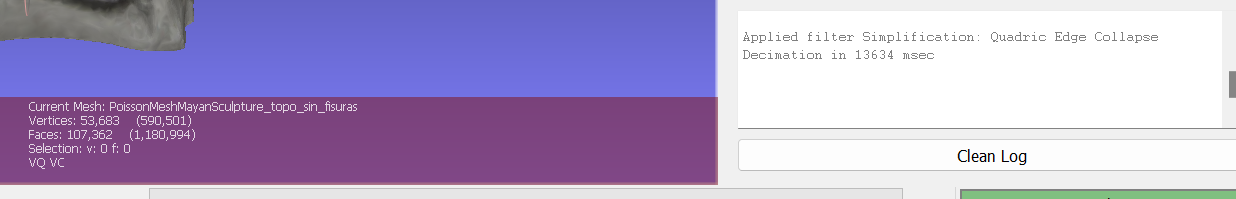
\includegraphics[scale=0.55]{images/simplificacion_02.png}
    \caption{Modelo reducido al 10\%}
\end{figure}

\subsubsection{Corrección topológica de la nueva malla}

Como tenemos un nuevo modelo, es necesario rehacer una comprobación topológica de los elementos. Como   

\paragraph{Comprobación de Autointersecciones}

Nos aparecen 4 caras, las identifico:

\begin{figure}[H]
    \centering
    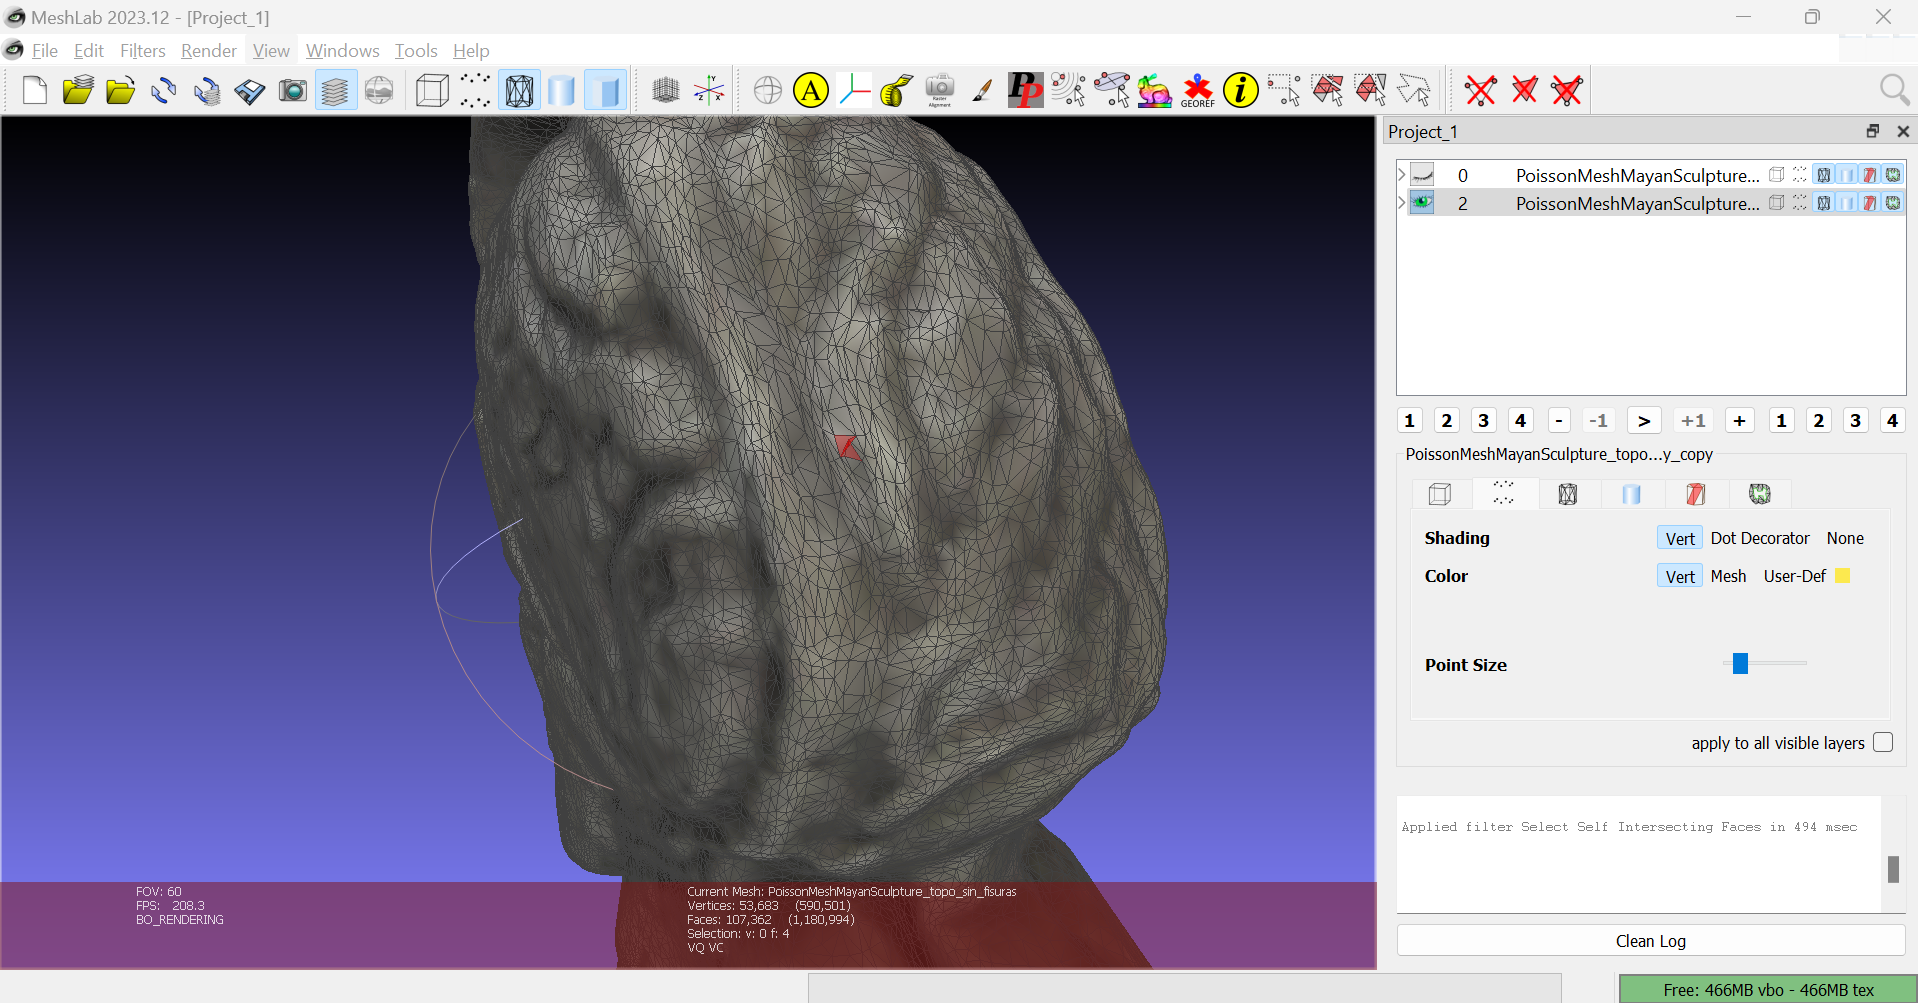
\includegraphics[scale=0.35]{images/simplificacion_03.png}
    \caption{Autointersecciones}
\end{figure}

Las elimino aprovechando la selección y cierro las fisuras generadas, estableciendo \textit{``Max size to be closed''} a 20. Las deselecciono y \textbf{vuelvo a lanzar el comprobador de autointersecciones}, resultando esta vez en \textbf{0}. Sigo con el resto de filtros de selección, pero no seleccionan nada:

\begin{itemize}
    \item Non Mainfold Edges
    \item Non Mainfold Vertices
\end{itemize}
~\\
Respecto al limpiado y reparación del modelo:

\begin{itemize}
    \item Remove T-Vertices
    \item Remove duplicate faces
    \item Remove duplicate vertices
    \item Remove isolated pieces (wrt Face Num.)
\end{itemize}

Durante estas acciones no se han eliminado vértices ni caras, de manera que tenemos el nuevo modelo simplificado topológicamente preparado.
Adjunto el detalle de la malla tras la simplificación:

\begin{figure}[H]
    \centering
    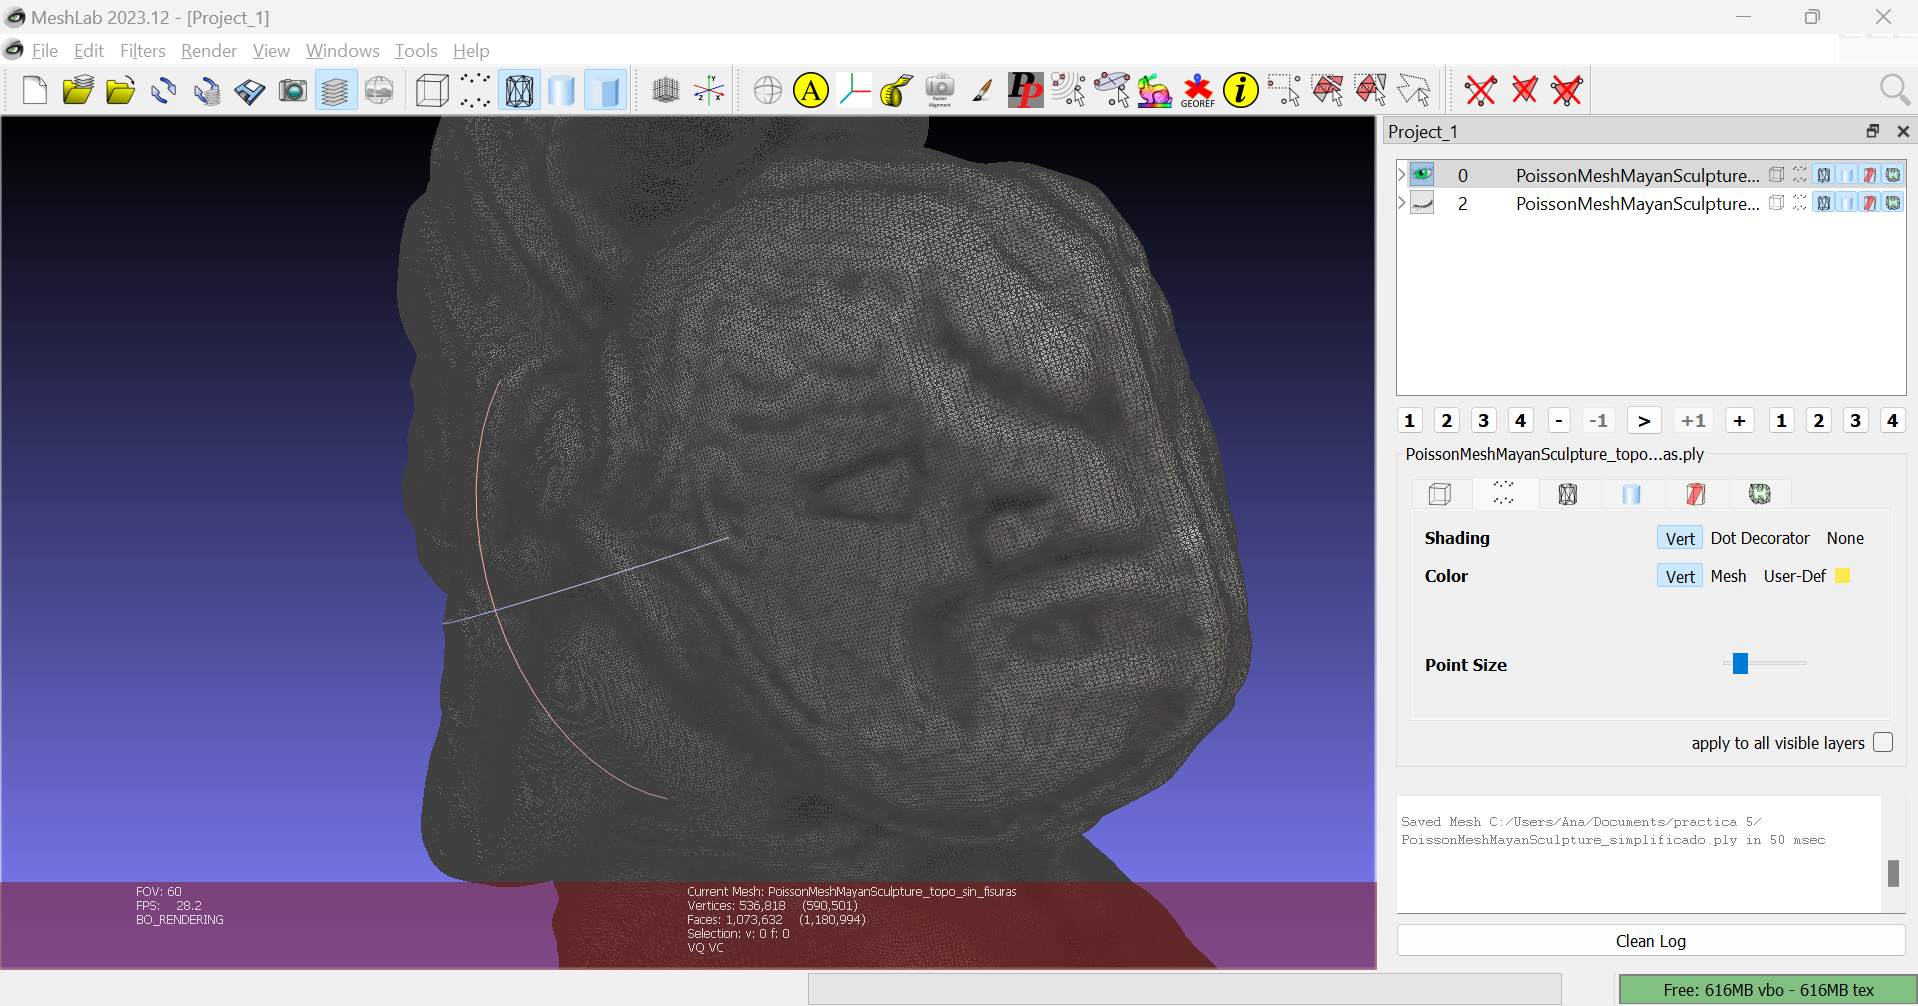
\includegraphics[scale=0.34]{images/simplificacion_04.png}
    \caption{Sin simplificación}
\end{figure}

\begin{figure}[H]
    \centering
    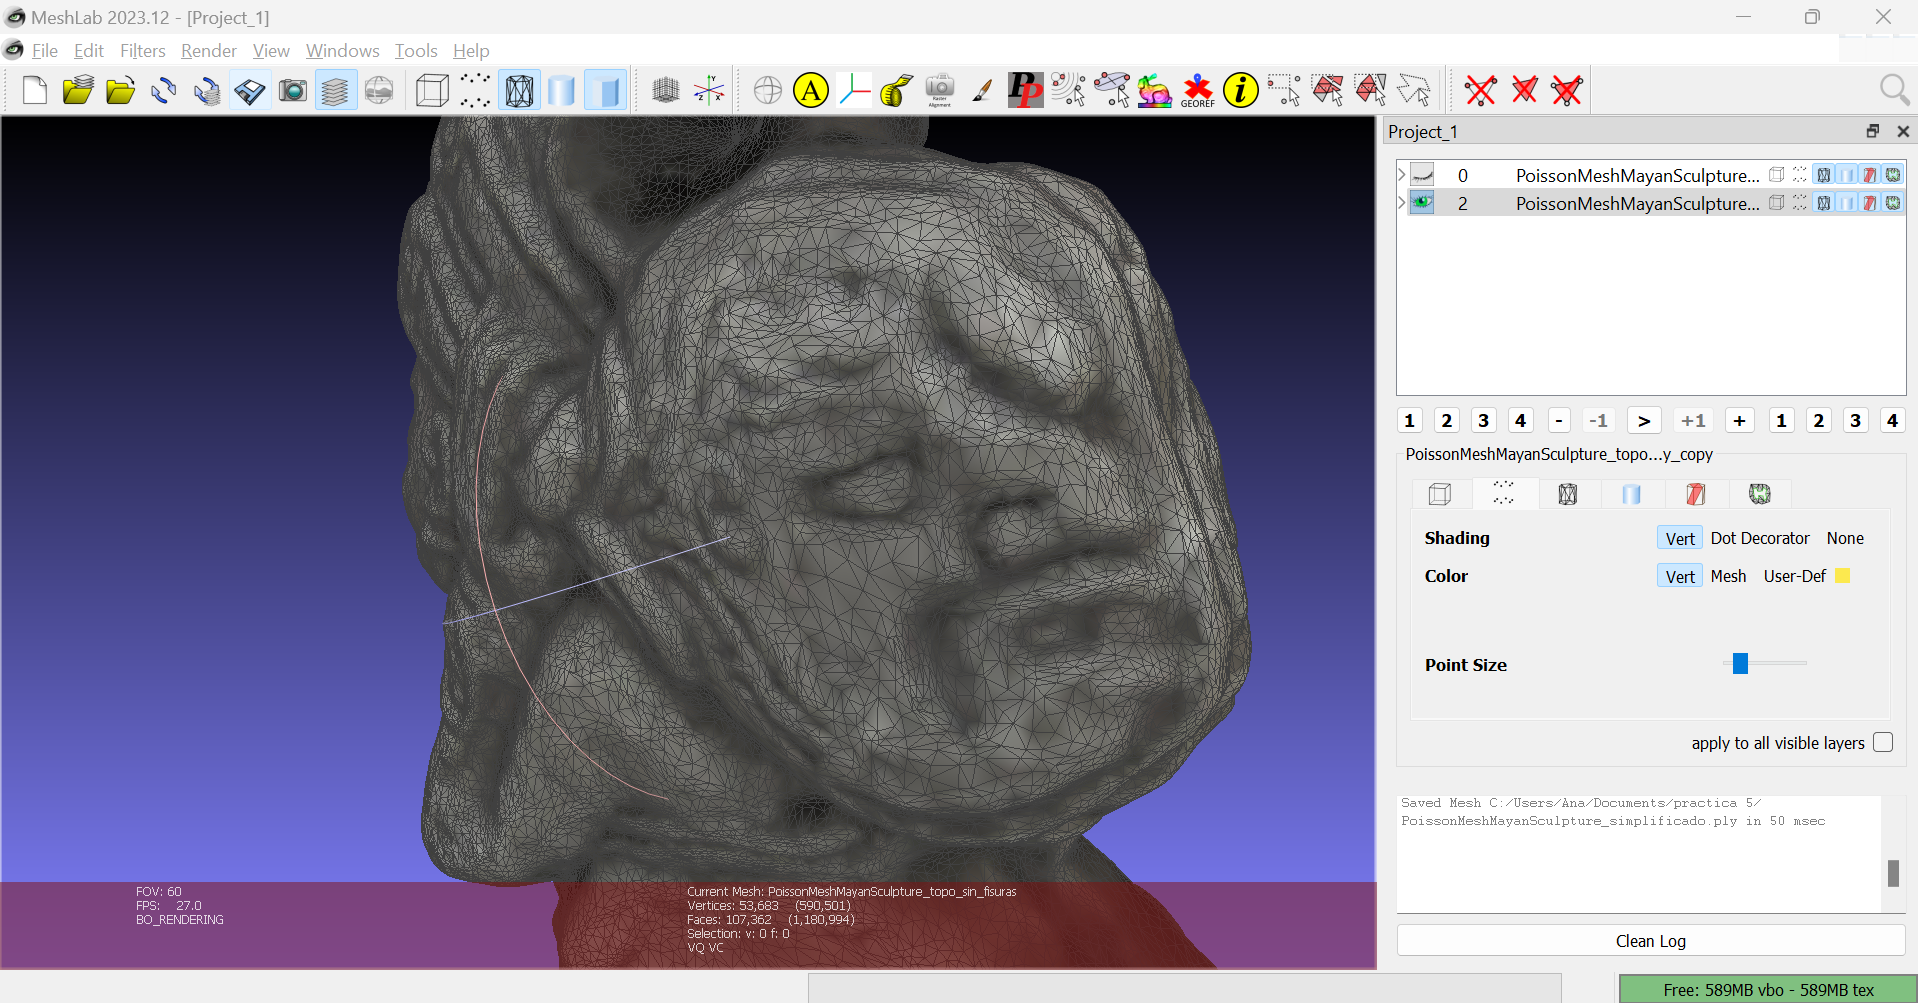
\includegraphics[scale=0.34]{images/simplificacion_05.png}
    \caption{Simplificada}
\end{figure}

\subsection{Parametrización}

Para realizar el \textit{``desenrollado''} de la malla y asginarle las coordenadas de textura de la pieza original, vamos a utilizar el algoritmo \textbf{Voronoy Atlas}. Para ello hacemos click en las siguientes secciones: \textbf{\textit{Filters → Texture → Parametrization: Voronoy Atlas}}. Se nos desplegará el siguiente panel, en el que haremos click en \textit{``Apply''}:

\begin{figure}[H]
    \centering
    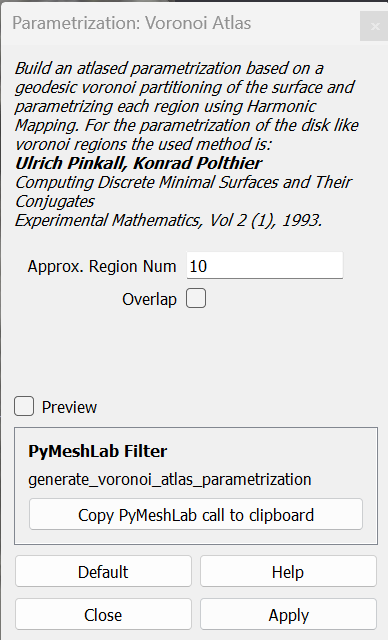
\includegraphics[scale=0.34]{images/parametrizacion_01.png}
    \caption{Panel Voronoy Atlas}
\end{figure}

Tras la ejecución, este es el resultado:

\begin{figure}[H]
    \centering
    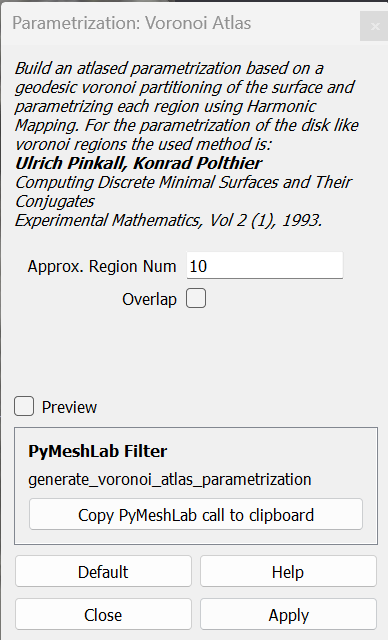
\includegraphics[scale=0.34]{images/parametrizacion_01.png}
    \caption{Panel Voronoy Atlas}
\end{figure}

\subsection{Texturización del modelo simplificado}

Dejo, para la comparación, la malla \textit{VoroAtlas} generada:

\begin{figure}[H]
    \centering
    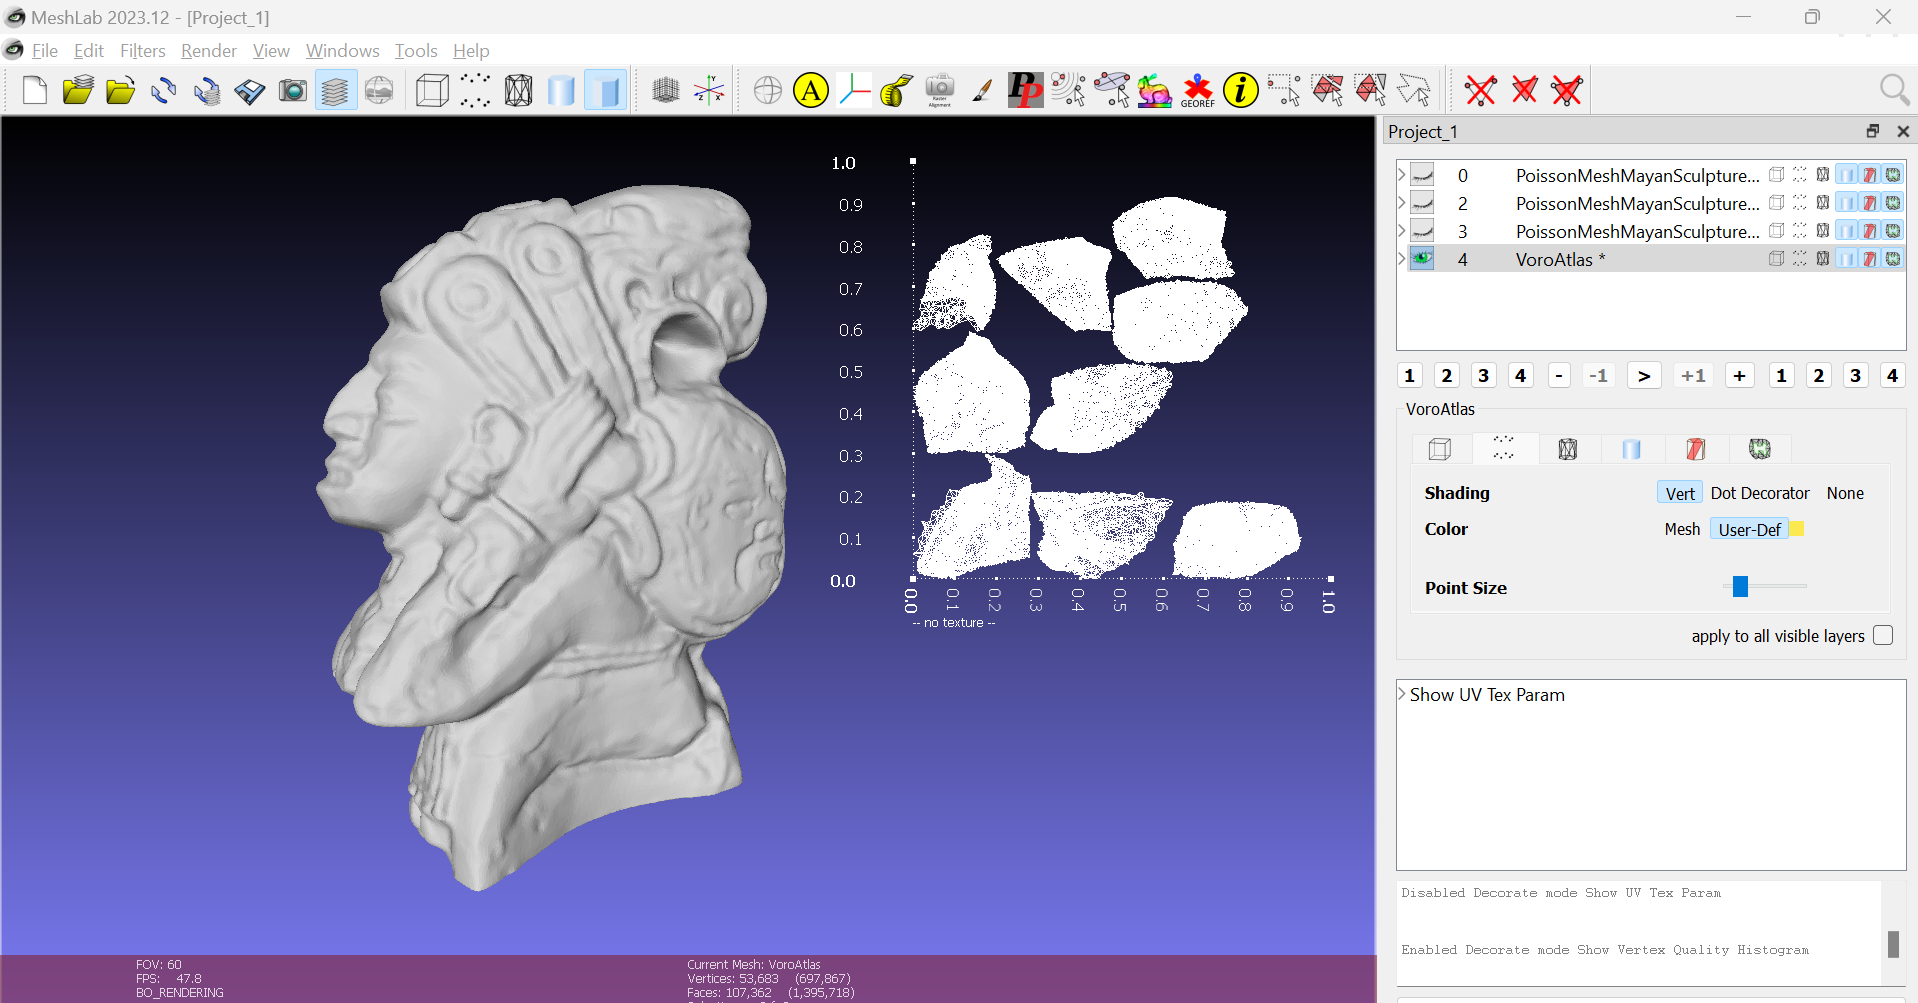
\includegraphics[scale=0.34]{images/textura_01.png}
    \caption{Voronoy Atlas antes de texturizar}
\end{figure}

Para transferir las texturas de la malla original al nuevo modelo simplificado utilizaremos la función, primero importo la malla de nube de puntos (la original), y luego utilizo la función: \textbf{\textit{Filters → Texture → Transfer: Vertex attributes to texture (1 or 2 meshes)}}. Se despliega el siguiente panel:

\begin{figure}[H]
    \centering
    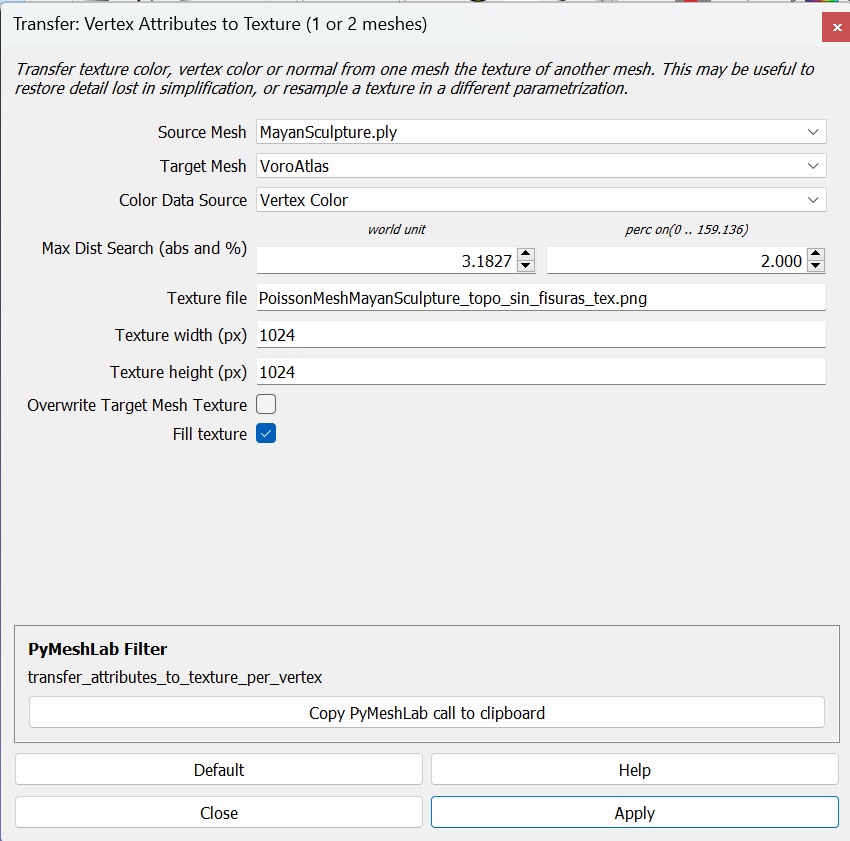
\includegraphics[scale=0.34]{images/textura_02.png}
    \caption{Panel de texturización}
\end{figure}

Este sería el resultado tras hacer click en \textit{``Apply''} y poner el color de las caras en blanco:

\begin{figure}[H]
    \centering
    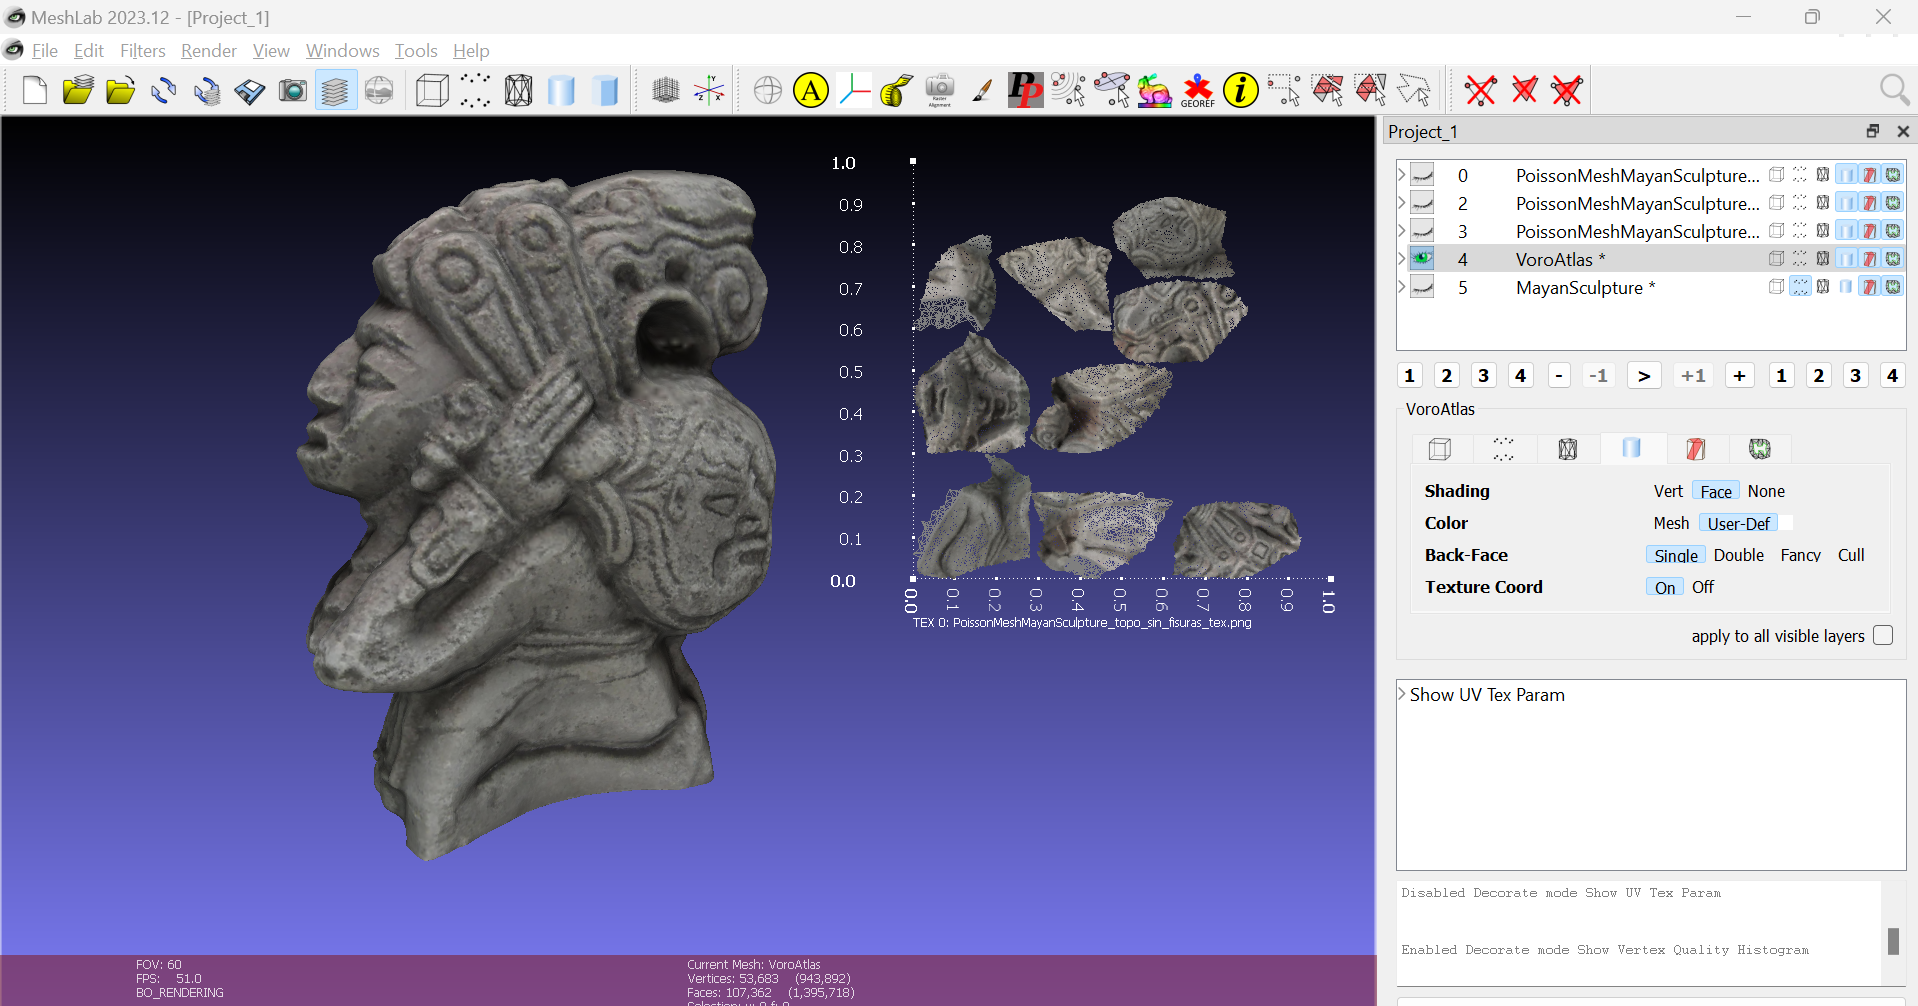
\includegraphics[scale=0.34]{images/textura_03.png}
    \caption{Modelo texturizado}
\end{figure}

Muestro el resultado de la textura en \texttt{.png}:

\begin{figure}[H]
    \centering
    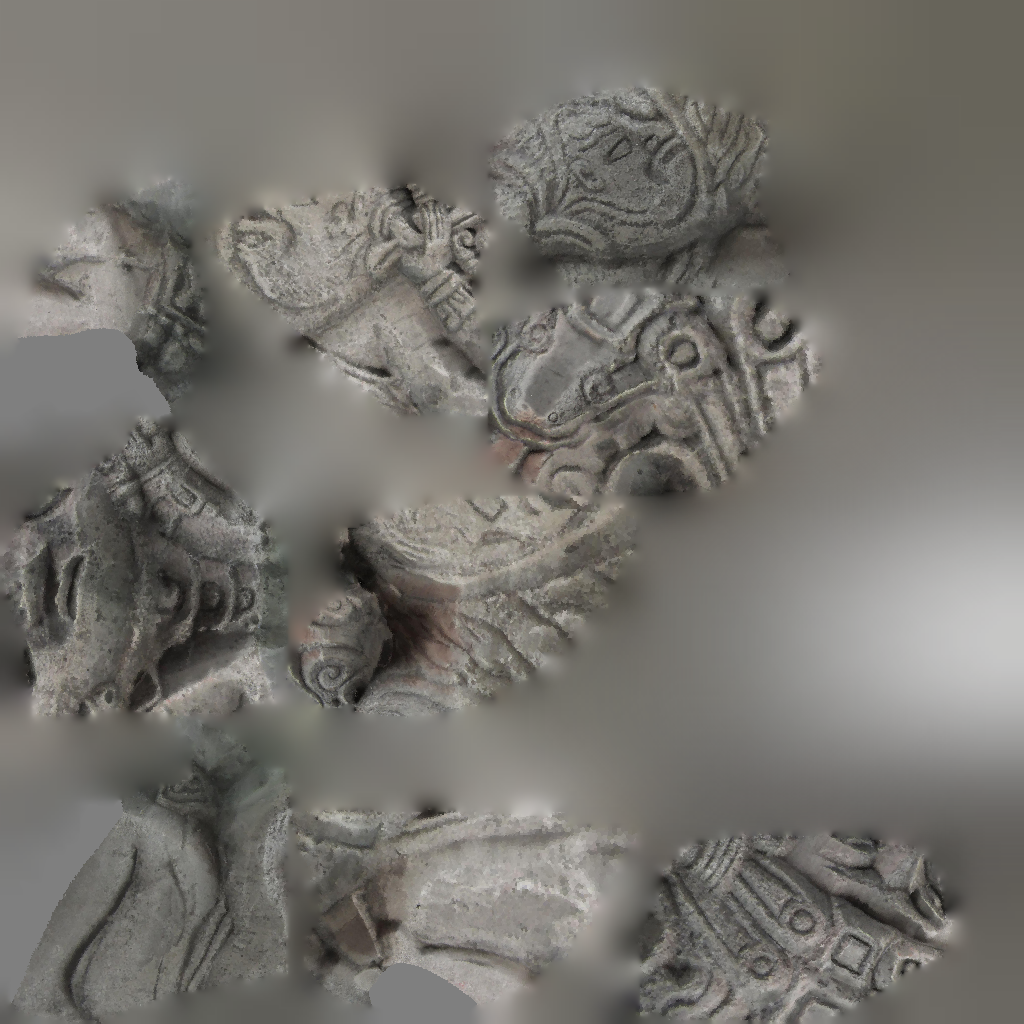
\includegraphics[scale=0.45]{images/PoissonMeshMayanSculpture_topo_sin_fisuras_tex.png}
    \caption{Modelo texturizado}
\end{figure}

\subsection{Publicación del modelo}

\subsubsection{Utilización de GitHub}

\textbf{GitHub} es una plataforma de colaboración en proyectos de software, apoyada en \textbf{Git}, lo cual nos permite llevar, además, un \textit{control de versiones} de los documentos que vayamos publicando en el repositorio. 


Para crear un repositorio y hacer seguimiento de este proyecto haremos click, dentro de nuestro panel principal, en \textbf{\textit{"New"}}:

\begin{center}
    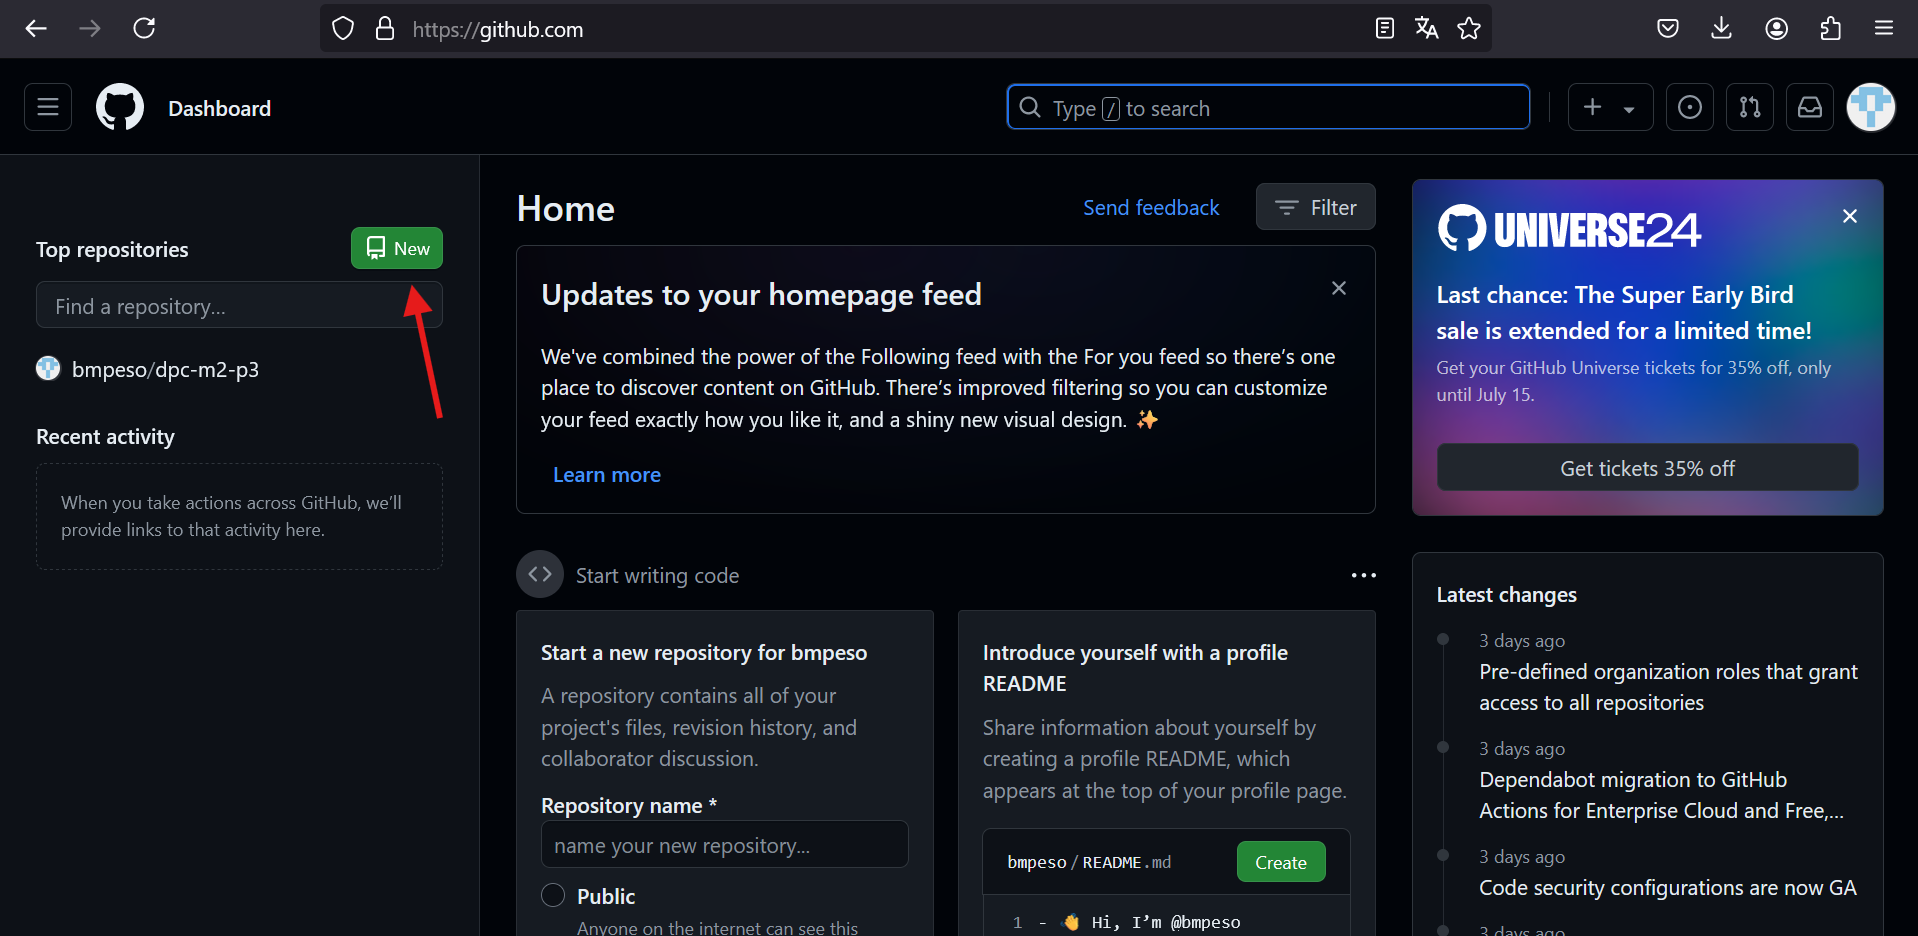
\includegraphics[scale=0.35]{images/github_01.png}
\end{center}

A continuación rellenaremos los campos que creamos convenientes \textit{(señalo en recuadros los campos modificados)} y haremos click en \textbf{\textit{Create repository}}:

\begin{center}
    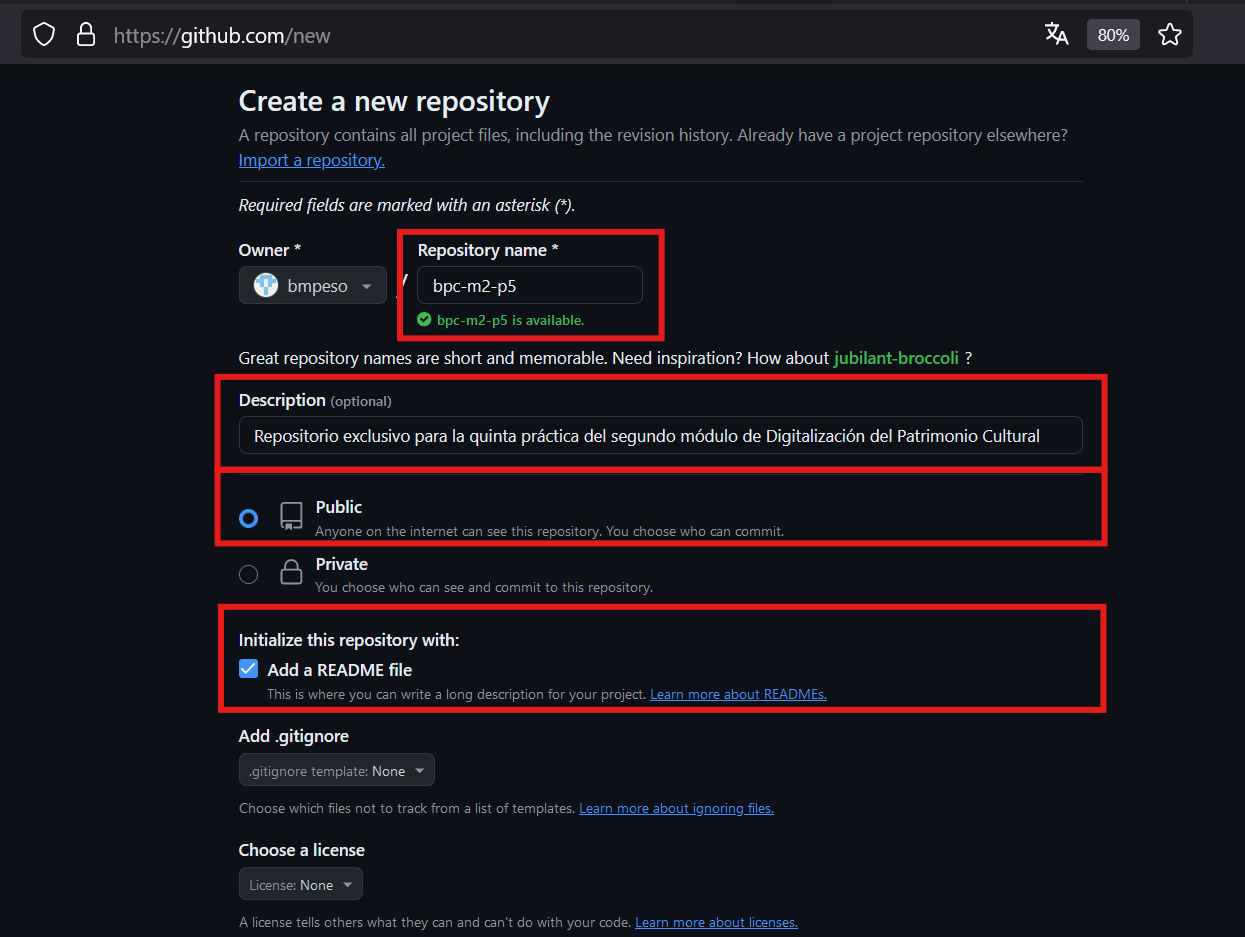
\includegraphics[scale=0.45]{images/github_02.png}
\end{center}


\end{document}